\documentclass[a4paper]{article}

%% Language and font encodings
\usepackage[english]{babel}
\usepackage[utf8x]{inputenc}
\usepackage[T1]{fontenc}

%% Sets page size and margins
\usepackage[a4paper,top=3cm,bottom=2cm,left=3cm,right=3cm,marginparwidth=1.75cm]{geometry}

%% Useful packages
\usepackage{amsmath}
\usepackage[colorinlistoftodos]{todonotes}
\usepackage[colorlinks=true, allcolors=blue]{hyperref}
\usepackage{graphicx}
\usepackage{listings}
\usepackage{subfig}
\usepackage{indentfirst}
\graphicspath{ {./images/} }
\lstset{language=R} 
\usepackage[super]{nth}

\title{Multivariate Analysis of Undocuments Immigrants in the United States}
\author{Harmit Chima, Amy Petris, Elizabeth Fabio}

\begin{document}
\maketitle

\section{Background}

The inspiration behind tracking a dataset from the 2019 Yearbook of Immigration Statistics (Department of Homeland Security) was from the Netflix documentary called “Immigration Nation”. The documentary takes a deep look into recent U.S. immigration policies and its effect on undocumented immigrants and their families. The 2020 documentary highlights everything related to U.S. immigration, from the duties of an Immigration and Customs Enforcement (ICE) officer to the criminalization of undocumented immigrants. \\

The documentary also goes into detail significant government policies that had a huge effect on undocumented immigrants. Figure \ref{fig:int_events} gives a timeline of these major immigration events and policies.

\begin{figure}[h!]
\centering

\includegraphics[scale=0.3]{images/int_events.jpg}
\caption{Major U.S. Immigration Policies}
\label{fig:int_events}
\end{figure}

\subsection{Data Source}

The \href{https://www.dhs.gov/immigration-statistics/yearbook/20192019}{Yearbook of Immigration Statistics} holds 41 tables that provides the number of immigrants in a variety of cases for each year. For example, some tables hold information regarding immigrants that were granted a green card or asylum/refugee status. Other tables, focused on this project, are related to immigration enforcement actions. These tables are:

\begin{itemize}
  \item \href{https://www.dhs.gov/immigration-statistics/yearbook/2019/table33}{Table 33. Aliens Apprehended: Fiscal Years 1925 to 2019}
  \item \href{https://www.dhs.gov/immigration-statistics/yearbook/2019/table39}{Table 39. Aliens Removed or Returned: Fiscal Years 1892 to 2019}
\end{itemize}

Table 33 is the number of immigrants apprehended each year from ICE or the U.S. Border Patrol. As for Table 39, it lists the number of immigrants deported. This table has two columns: (1) immigrants deported based on an order of removal and (2) immigrants deported not based on an order of removal. The website was not clear regarding what was the difference between deportation based an order of removal and not from an order of removal. But from our understanding, an order of removal means that  undocumented immigrants went through immigration court to make a plea. As for immigrants deported not due to an order of removal, this means that they voluntarily chose to be deported and to not go through the immigration court process. \\

After copying and pasting these tables into a CSV file, they were uploaded into Kaggle as public datasets:

\begin{itemize}
    \item \href{https://www.kaggle.com/ekayfabio/immigration-apprehended}{Undocumented Immigrants Apprehended in the U.S.}
    \item \href{https://www.kaggle.com/ekayfabio/immigration-deported}{Undocumented Immigrants Deported in the U.S.}
\end{itemize}

After loading the two CSV files in R, we defined the datasets to the following variables:

\begin{itemize}
    \item \textbf{num}: Number of Undocumented Immigrants Apprehended
    \item \textbf{rem}: Number of Undocumented Immigrants Deported Based on a Order of Removal
    \item \textbf{ret}: Number of Undocumented Immigrants Deported Not Based on a Order of Removal
\end{itemize}

\subsection{Statistics}
%example of how to include images
%just makes sure the image is in the images folder
\begin{table}[h!]
    \centering
    \caption{Basic Summary Statistics}
    \begin{tabular}{|c|c|c|c|}
    \hline
    & Mean & Median & Standart Deviation \\
    \hline
    Apprehended & $614,880.9$ & $530,250$ & $543,896$ \\ 
    \hline
    Removed & $67,906.48$ & $19,312$ & $112,950.2$ \\
    \hline
    Returned & $521,888.5$ & $30,3348$ & $501,417.5$ \\ 
    \hline
    \end{tabular}
    \label{tab:lambda}
\end{table}

\subsection{Presidential Analysis}


\begin{figure}[h!]
\centering
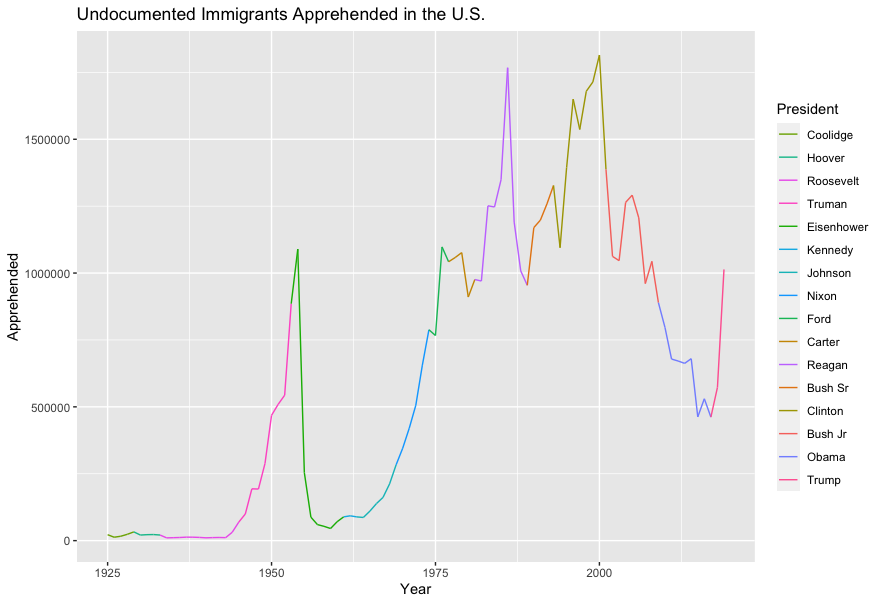
\includegraphics[scale=0.3]{images/presapp.png}
\caption{Time Series Plot of Apprehended by President}
\label{fig:pres_app}
\end{figure}

The \nth{42} president, Bill Clinton, had the highest number of undocumented immigrants apprehended during his terms with an average of $1,526,405.4$ immigrants apprehended each year from 1993 to 2001. The \nth{32} president, Franklin D. Roosevelt, had the lowest average number of immigrants apprehended with approximately 13989.4 immigrants apprehended each year between 1933 and 1945. \\

\begin{figure}[h!]
\centering
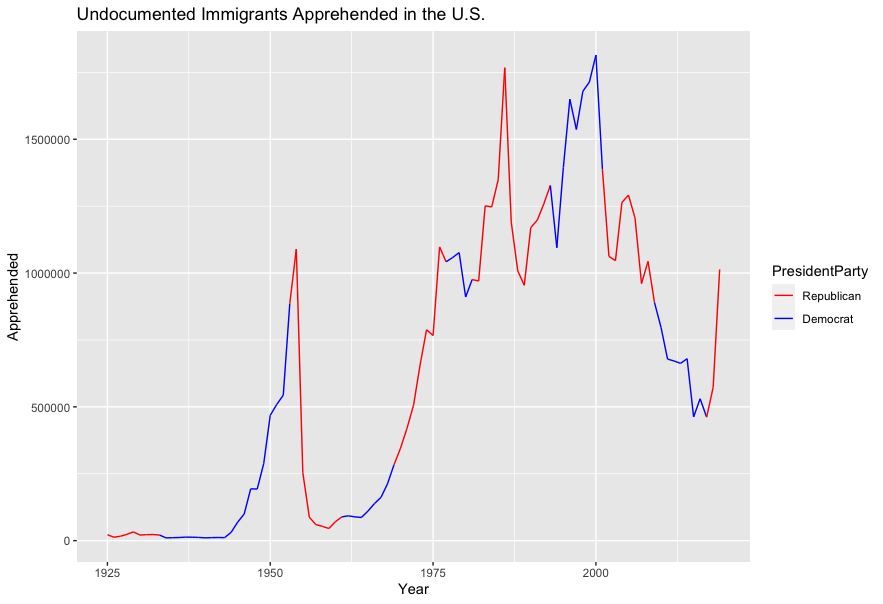
\includegraphics[scale=0.3]{images/partyapp.png}
\caption{Time Series Plot of Apprehended by President Party}
\label{fig:party_app}
\end{figure}

On average, 707,084 immigrants are apprehended under a Republican president, while 524,599 are apprehended under a Democratic president.


\section{Model Building}

For determining the model order, the following steps need to be taken:

\begin{enumerate}
  \item \textbf{Check Stationarity}: You can check a dataset is stationary either by analyzing visualizations or through hypothesis testing. The visualizations to refer to are time series plots, autocorrelation function (ACF) plots, and partial autocorrelation function (PACF) plots. As for hypothesis testing, we can perform the augmented Dickey-Fuller unit-root test and the Box Cox transformation function to determine stationarity.
  \item \textbf{Perform Data Transformation}: If a dataset is not stationary, the dataset needs to be applied with a log transformation and/or differenced. If the data has a non-constant mean, then we only need to take the difference. If the data has a non-constant variance, then the data needs to be applied with a log transformation. However, if the data has both a non-constant mean and a non-constant variance, then a log transformation needs to be applied first and then we can take the difference.
  \item \textbf{Determine a Set of Preliminary Models}: Based on the ACF and PACF we can determine the autoregressive (AR) or the moving average (MA) order based on where the lag cuts off. We can also use the extended autocorrelation function (EACF) to determine the ARMA model as well.
  \item \textbf{Select the Best Model Order}: Calculate the Akaike information criterion (AIC) for each model in question. The AIC is a measurement of how well the data fits the model. Essentially the best fit model has the smallest AIC value. Thus, the model with the lowest AIC is  selected.
  \item \textbf{Determine Coefficient Significance}: Apply the model into an ARIMA function in R and use the coeftest function to gain inference on the estimated coefficients. Create a new ARIMA model with only the significant coefficients and compare it with the original model. Select the model with the lowest AIC value.
\end{enumerate}

\subsection{Determine Model Order}
Each model order will be determined for the three datasets (num, ret, rem).\\

\subsubsection{Check Stationarity}
First, we plot the time series and note any trends (Figures \ref{fig:ts_app} \& \ref{fig:ts_dep}).

\begin{figure}[h!]
\centering
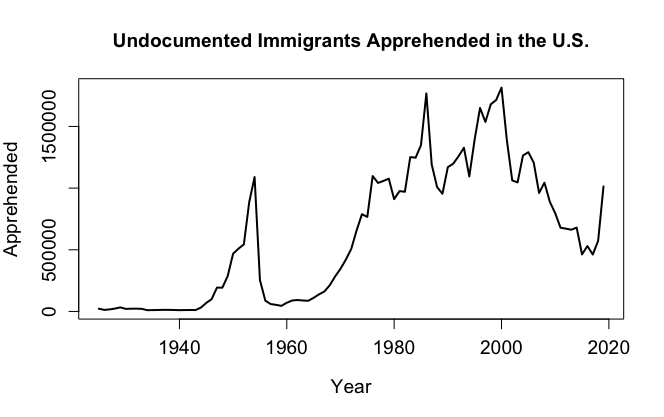
\includegraphics[scale=0.4]{images/ts_apprehended.png}
\caption{Time Series Plot of num}
\label{fig:ts_app}
\end{figure}

\begin{figure}[h!]
\centering
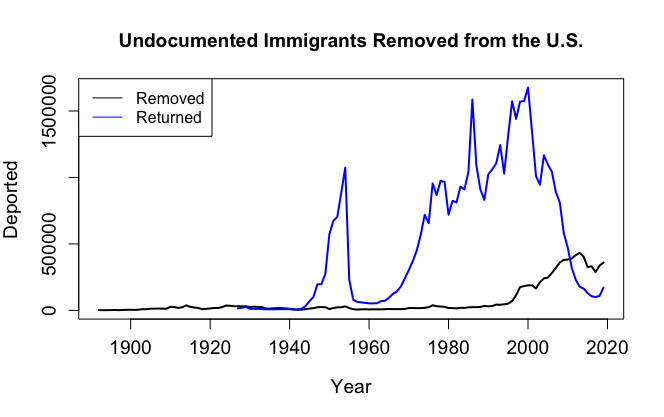
\includegraphics[scale=0.4]{images/ts_deported.png}
\caption{Time Series Plot of rem and ret}
\label{fig:ts_dep}
\end{figure}

Both plots appear to have a non-constant variance considering there are several spikes especially around 1950 and near the early 2000s. As for non-constant variance, the datasets does not appear to need a log transformation. However, further tests needs to be done to confirm.\\

\begin{figure}[h!]
\centering
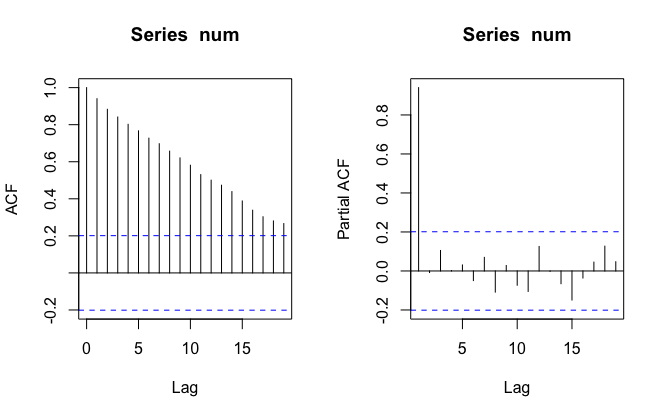
\includegraphics[scale=0.4]{images/acf_pacf_num.png}
\caption{ACF \& PACF of num}
\label{fig:acf_pacf_num}
\end{figure}

\begin{figure}[h!]
\centering
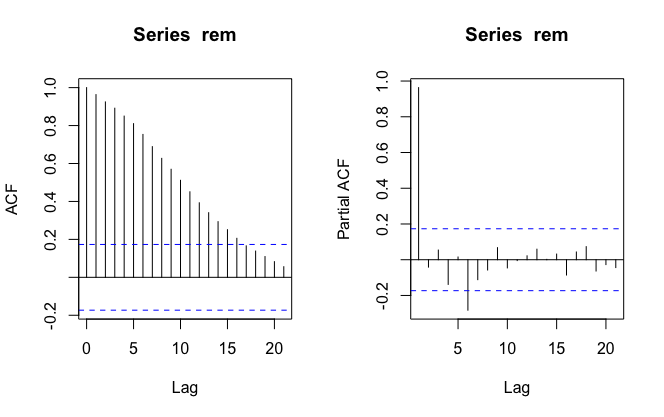
\includegraphics[scale=0.4]{images/acf_pacf_rem.png}
\caption{ACF \& PACF of rem}
\label{fig:acf_pacf_rem}
\end{figure}

\begin{figure}[h!]
\centering
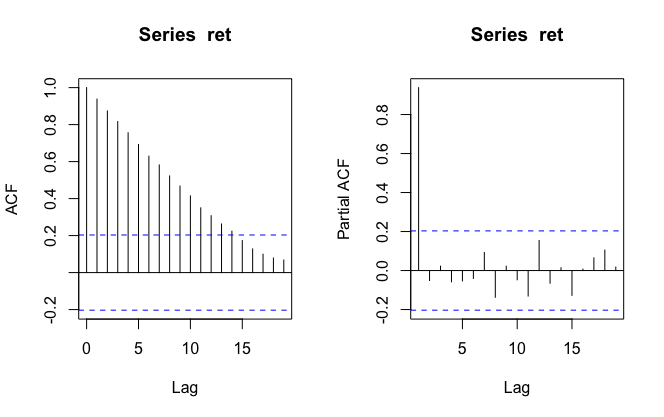
\includegraphics[scale=0.4]{images/acf_pacf_ret.png}
\caption{ACF \& PACF of ret}
\label{fig:acf_pacf_ret}
\end{figure}

Next, we plot the ACF and PACF for each of the three datasets (Figures \ref{fig:acf_pacf_num}, \ref{fig:acf_pacf_rem}, \& \ref{fig:acf_pacf_ret}). The ACF and PACF of all three datasets appear to have the lag tail off in the ACF plot while the PACF plot cuts off at lag 1. This shows that the models are currently AR. However, it is still hard to determine if the models are stationary just by those plots alone. Further proof from getting the roots of these AR models would be necessary.\\

Compared to using the visualization plots, we can use a variety of tests and functions to confirm the data's stationarity. For instance, using the BoxCox.lambda function in R predicts the lambda value. If lambda is close to zero, then a log transformation is needed. After applying the function to all three datasets, we have the following lambda values listed in Table \ref{tab:lambda}. \\

\begin{table}[h!]
    \centering
    \caption{BoxCox.lambda Function Lambda Values}
    \begin{tabular}{|c|c|c|}
    \hline
    Dataset & Lambda & Log Transformation Needed? \\
    \hline
    num & -0.139 & Yes \\ 
    \hline
    rem & 0.172 & Yes \\
    \hline
    ret & -0.042 & Yes \\ 
    \hline
    \end{tabular}
    \label{tab:lambda}
\end{table}

To determine if the data needs to be differenced, we can use the augmented Dickey-Fuller unit-root test. The following conditions for this test are:

\begin{itemize}
    \item \underline{$H_0$}: ARIMA(p, d, q) process with $d \neq 0$ (Data is not stationary).
    \item \underline{$H_a$}: ARIMA(p, d, q) process with $d =  0$ (Data is stationary).
    \item \underline{Condition}: Reject $H_0$ if p-value is less than 0.05. This means if the p-value is greater than 0.05, the data is not stationary and needs to be differenced.
\end{itemize}

For the results from the augmented Dickey-Fuller unit root test for each dataset refer to Table \ref{tab:dickey1}.

\begin{table}[h!]
    \centering
    \caption{Augmented Dickey-Fuller Unit-Root Test p-Values}
    \begin{tabular}{|c|c|c|}
    \hline
    Dataset & p-Value & Difference Needed? \\
    \hline
    num & 0.2082 & Yes \\ 
    \hline
    rem & 0.7145 & Yes \\
    \hline
    ret & 0.3364 & Yes \\ 
    \hline
    \end{tabular}
    \label{tab:dickey1}
\end{table}

\subsubsection{Perform Data Transformation}
After applying the log transformation first and then differencing the data, we have the following time series plots (Figure \ref{fig:ts_app_trans} \& \ref{fig:ts_dep_trans}) and ACF and PACF plots (Figure \ref{fig:acf_pacf_dlognum}, \ref{fig:acf_pacf_dlogrem}, \& \ref{fig:acf_pacf_dlogret}) for our three datasets. \\

The following variables represent the log transformed and differenced dataset:

\begin{itemize}
    \item \textbf{dlognum}: Transformed num Dataset
    \item \textbf{dlogrem}: Transformed rem Dataset
    \item \textbf{dlogret}: Transformed ret Dataset
\end{itemize}

\begin{figure}[h!]
\centering
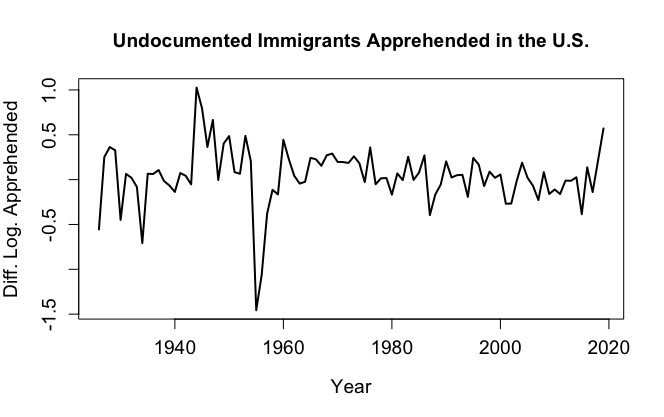
\includegraphics[scale=0.4]{images/ts_app_trans.png}
\caption{Time Series Plot of dlognum}
\label{fig:ts_app_trans}
\end{figure}

\begin{figure}[h!]
\centering
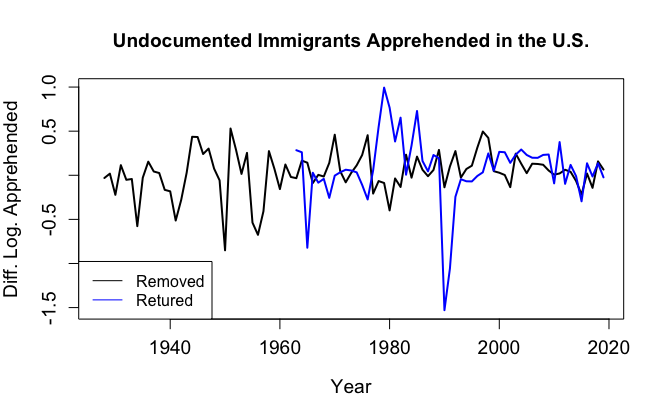
\includegraphics[scale=0.4]{images/ts_dep_trans.png}
\caption{Time Series Plot of dlogrem and dlogret}
\label{fig:ts_dep_trans}
\end{figure}

\begin{figure}[h!]
\centering
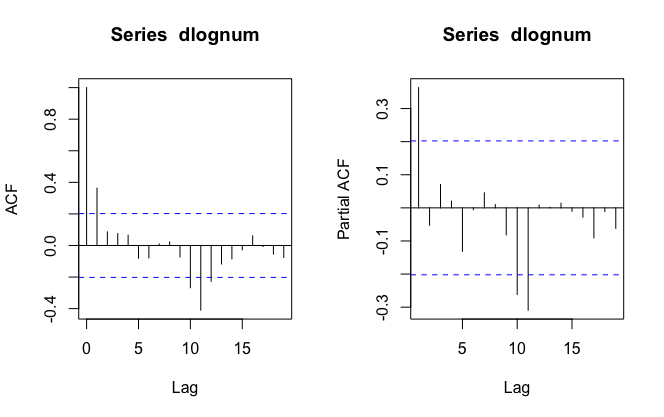
\includegraphics[scale=0.4]{images/acf_pacf_dlognum.png}
\caption{ACF \& PACF of dlognum}
\label{fig:acf_pacf_dlognum}
\end{figure}

\begin{figure}[h!]
\centering
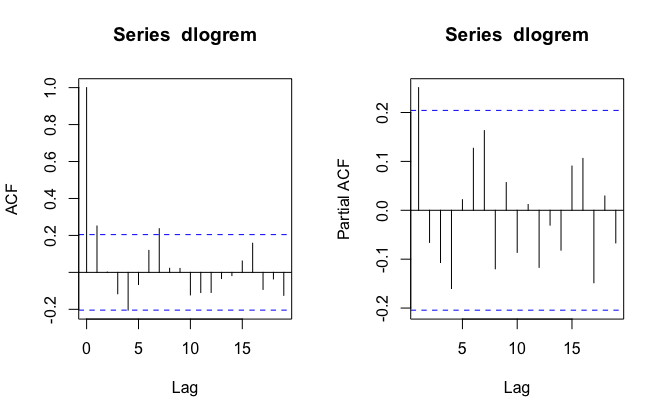
\includegraphics[scale=0.4]{images/acf_pacf_dlogrem.png}
\caption{ACF \& PACF of dlogrem}
\label{fig:acf_pacf_dlogrem}
\end{figure}

\begin{figure}[h!]
\centering
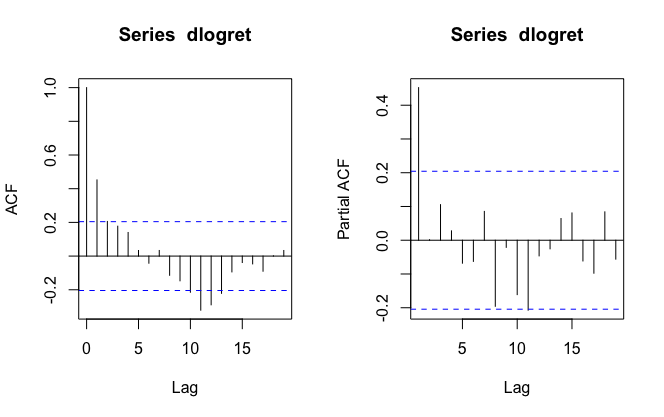
\includegraphics[scale=0.4]{images/acf_pacf_dlogret.png}
\caption{ACF \& PACF of dlogret}
\label{fig:acf_pacf_dlogret}
\end{figure}

Minus the outliers, our time series plots appear to be stationary along with the ACF and PACF plots. The time series plots do not have a general trend and the ACF and PACF plots have lags that are not not significant (within the dotted blue line).\\

To further confirm the newly transformed datasets are stationary, we performed the augmented Dickey-Fuller unit root test. The results are listed in Table \ref{tab:dickey2}.

\begin{table}[h!]
    \centering
    \caption{Augmented Dickey-Fuller Unit-Root Test p-Values on Transformed Data}
    \begin{tabular}{|c|c|c|}
    \hline
    Dataset & p-Value & Difference Needed? \\
    \hline
    dlognum & <0.01 & No \\ 
    \hline
    dlogrem & <0.01 & No \\
    \hline
    dlogret & 0.04066 & No \\ 
    \hline
    \end{tabular}
    \label{tab:dickey2}
\end{table}

\subsubsection{Determine a Set of Preliminary Models}

We can refer to the ACF and PACF plots in Figures \ref{fig:acf_pacf_dlognum}, \ref{fig:acf_pacf_dlogrem}, and \ref{fig:acf_pacf_dlogret} to make an inference regarding their model orders. For easier interpretation we used the EACF plot as well. To determine a model order on an EACF plot, we traced over a triangle of 0's that line the border. The better model is where the triangle index is closest to the top-left corner. In Figure \ref{fig:eacf_num}, \ref{fig:eacf_rem}, and \ref{fig:eacf_ret}, the 0's highlighted in blue are the borders of the triangle. \\

Two triangles were selected in Figure \ref{fig:eacf_num}. One triangle is where the index is at MA(12) and another is where the index is at ARMA(1,11). The reason why two triangles were selected instead of one is because MA(12) and ARMA(1,11) are close together. It would be hard to determine which model is the best unless its tested further. \\

\begin{figure}[h!]
\centering
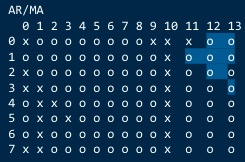
\includegraphics[scale=0.6]{images/eacf_num.jpg}
\caption{EACF of dlognum}
\label{fig:eacf_num}
\end{figure}

\begin{figure}[h!]
\centering
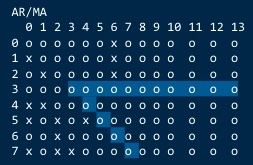
\includegraphics[scale=0.57]{images/eacf_rem.jpg}
\caption{EACF of dlogrem}
\label{fig:eacf_rem}
\end{figure}

\begin{figure}[h!]
\centering
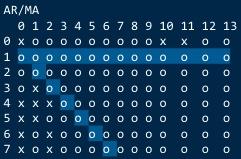
\includegraphics[scale=0.6]{images/eacf_ret.jpg}
\caption{EACF of dlogret}
\label{fig:eacf_ret}
\end{figure}

So based on our EACF plots the model orders to test are:

\begin{itemize}
    \item \textbf{num}: MA(12) and ARMA(1,11)
    \item \textbf{rem}: ARMA(3,3)
    \item \textbf{ret}: AR(1)
\end{itemize}

\subsubsection{Select the Best Model Order}

To select the best model order, an ARIMA model is created in R. We then compare the AIC values for each model and select the model order with the smallest AIC value. Since only the num dataset has two possible models, we only created the ARIMA models for that dataset and calculated the AIC values listed in Table \ref{tab:aic1}. \\

\begin{table}[h!]
    \centering
    \caption{AIC Model Selection of dlognum}
    \begin{tabular}{|c|c|c|}
    \hline
    Model Order & AIC & Model Selected? \\
    \hline
    MA(12) & 47.24 & No \\ 
    \hline
    ARMA(1,11) & 46.53 & Yes \\
    \hline
    \end{tabular}
    \label{tab:aic1}
\end{table}

\subsubsection{Determine Coefficient Significance}
\label{section:coef}

Next, we can compare the AIC values of ARIMA models that have only their significant coefficients. We first begin with using the coeftest function in R to determine each significant coefficient within the 95\% confidence interval. Next, we created another ARIMA model with the same order but only having their significant variables selected. Then we compared the two similar models and chose the one with the best AIC value. \\

In Table \ref{tab:aic2}, we listed each possible model along with its AIC values. For the num dataset, we checked again MA(12) with only the significant coefficients even though ARMA(1,11) was originally selected.

\begin{table}[h!]
    \centering
    \caption{Final AIC Model Selection}
    \begin{tabular}{|c|c|c|c|c|}
    \hline
    Dataset & Model Order & Significant Coefficients Only? & AIC & Model Selected? \\
    \hline
    num & ARMA(1,11) & No & 44.53 & No \\
    \hline
    num & ARMA(1,11) & Yes & 38.00 & No \\
    \hline
    num & MA(12) & No & 45.24 & No \\
    \hline
    num & MA(12) & Yes & 32.97 & Yes \\
    \hline
    rem & ARMA(3,3) & No &  26.75 & Yes \\
    \hline
    rem & ARMA(3,3) & Yes & 30.06 & No \\
    \hline
    ret & AR(1) & No &  41.05 & No \\
    \hline
    ret & AR(1) & Yes &  39.38 & Yes \\
    \hline
    \end{tabular}
    \label{tab:aic2}
\end{table}

\subsection{Model Diagnostics}

Before using the selected model order for further analysis, we need to perform the following diagnostic steps:
\begin{enumerate}
  \item \underline{Step 1}: Perform residual analysis to check for underspecification.
  \item \underline{Step 2}: Check for overspecification. This is performed in the last step already when determining the model order (Section \ref{section:coef}).
  \item \underline{Step 3}: Check for stationarity through the AR roots.
  \item \underline{Step 4}: Check for model redundancy through the AR and MA roots.
\end{enumerate}

\subsubsection{Residual Analysis - Underspecification}
For the residual analysis, the time series and the ACF and PACF were plotted first. The time series residual plots can be seen in Figure \ref{fig:res_num}, \ref{fig:res_rem}, and \ref{fig:res_ret}, and the ACF and PACF residual plots can be seen in Figure \ref{fig:res_acf_pacf_num}, \ref{fig:res_acf_pacf_rem}, and \ref{fig:res_acf_pacf_ret}.

\begin{figure}[h!]
\centering
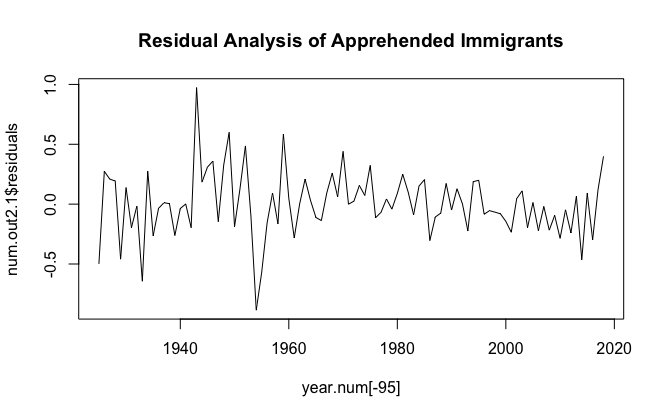
\includegraphics[scale=0.4]{images/residual_num.png}
\caption{Residual Time Series Plot of num MA(12) Model with Significant Coefficients Only}
\label{fig:res_num}
\end{figure}

\begin{figure}[h!]
\centering
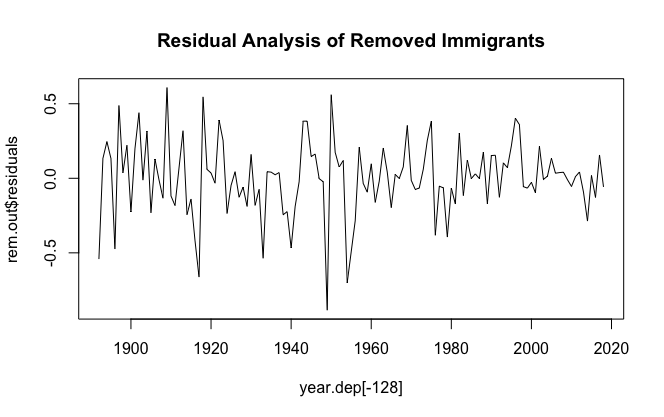
\includegraphics[scale=0.4]{images/residual_rem.png}
\caption{Residual Time Series Plot of rem ARMA(3,3) Model}
\label{fig:res_rem}
\end{figure}

\begin{figure}[h!]
\centering
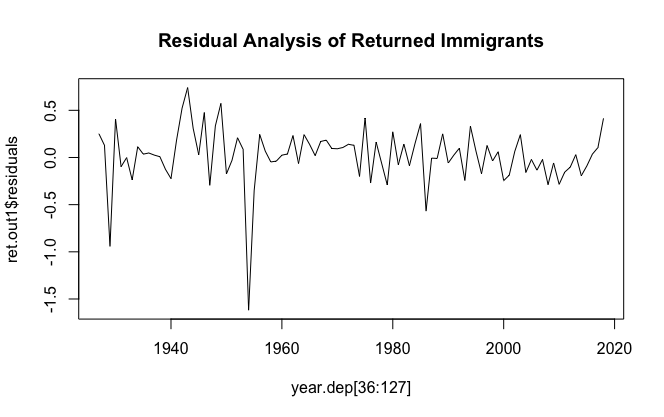
\includegraphics[scale=0.4]{images/residual_ret.png}
\caption{Residual Time Series Plot of ret AR(1,1) Model with Significant Coefficients Only}
\label{fig:res_ret}
\end{figure}

\begin{figure}[h!]
\centering
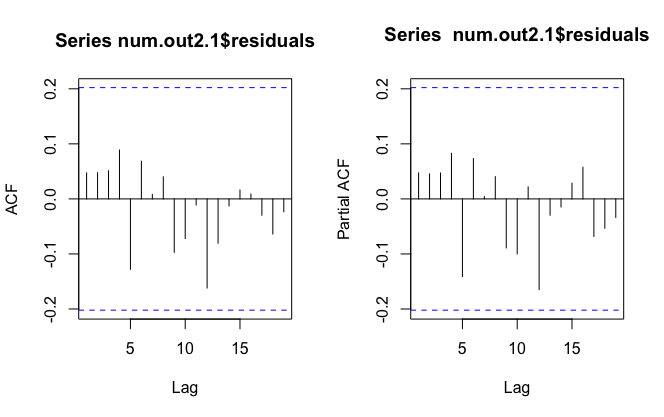
\includegraphics[scale=0.4]{images/res_acf_pacf_num.png}
\caption{Residual ACF \& PACF of num MA(12) With Significant Coefficients Only}
\label{fig:res_acf_pacf_num}
\end{figure}

\begin{figure}[h!]
\centering
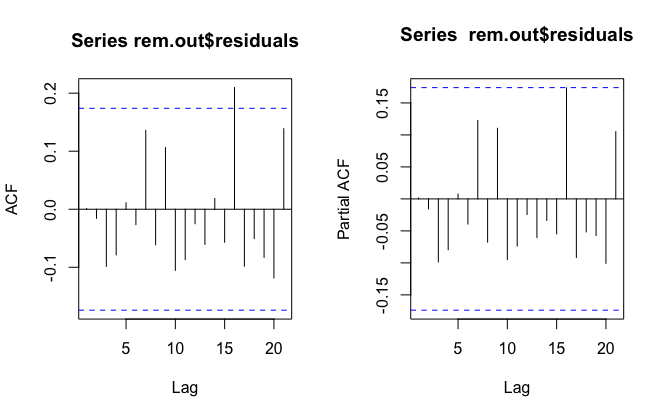
\includegraphics[scale=0.4]{images/res_acf_pacf_rem.png}
\caption{Residual ACF \& PACF of rem ARMA(3,3) Model}
\label{fig:res_acf_pacf_rem}
\end{figure}

\begin{figure}[h!]
\centering
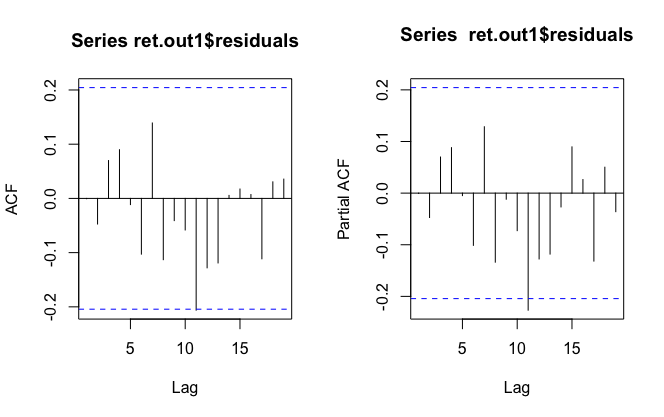
\includegraphics[scale=0.4]{images/res_acf_pacf_ret.png}
\caption{Residual ACF \& PACF of ret AR(1,1) Model with Significant Coefficients Only}
\label{fig:res_acf_pacf_ret}
\end{figure}

The residual time series plots for all the datasets appears to be generally white noise as well as the ACF and PACF plots. To confirm if the residuals for the selected models are white noise, we can perform the Box-Ljung test. The conditions for this test are:

\begin{itemize}
    \item \underline{$H_0$}: $\rho_1=\rho_2=...=0$ (white noise)
    \item \underline{$H_a$}: At least one $\rho_k\neq0$ (not white noise)
    \item \underline{Condition}: Reject $H_0$ if p-value is less than 0.05. This means if the p-value is greater than 0.05 the residuals are not white noise.
\end{itemize}

All the models' residuals are white noise based on their p-values listed in Table \ref{tab:ljung}. Thus, our selected models are not underspecified.

\begin{table}[h!]
    \centering
    \caption{Box-Ljung Test p-Values}
    \begin{tabular}{|c|c|c|c|}
    \hline
    Dataset & Model & p-Value & Residual Are White Noise? \\
    \hline
    num & MA(12) With Significant Coefficients Only &  0.7654 & Yes \\ 
    \hline
    rem & ARMA(3,3) &  0.6548 & Yes \\
    \hline
    ret & AR(1) With Significant Coefficients Only & 0.3927 & Yes \\ 
    \hline
    \end{tabular}
    \label{tab:ljung}
\end{table}

\subsubsection{Overspecfication}
The coeftest output for each model order along with the model orders with only the significant coefficients is listed below. To see which model was selected, refer to Section \ref{section:coef}.\\

\textbf{Coeftest Output for MA(12) - num Dataset}

\begin{verbatim}
z test of coefficients:

           Estimate Std. Error z value  Pr(>|z|)    
ma1        0.341711   0.127292  2.6845 0.0072644 ** 
ma2       -0.010666   0.131395 -0.0812 0.9353046    
ma3       -0.023095   0.164579 -0.1403 0.8884000    
ma4        0.143448   0.143925  0.9967 0.3189148    
ma5       -0.070559   0.159197 -0.4432 0.6576104    
ma6       -0.413222   0.159013 -2.5987 0.0093585 ** 
ma7       -0.091808   0.123955 -0.7407 0.4589009    
ma8       -0.020123   0.130787 -0.1539 0.8777163    
ma9       -0.073581   0.151119 -0.4869 0.6263233    
ma10      -0.029191   0.127751 -0.2285 0.8192582    
ma11      -0.572337   0.168295 -3.4008 0.0006719 ***
ma12      -0.180392   0.160995 -1.1205 0.2625080    
intercept  0.049395   0.010147  4.8681 1.127e-06 ***
---
Signif. codes:  0 ‘***’ 0.001 ‘**’ 0.01 ‘*’ 0.05 ‘.’ 0.1 ‘ ’ 1
\end{verbatim}

\textbf{Coeftest Output for MA(12) Significant Coefficients Only - num Dataset}

\begin{verbatim}
z test of coefficients:

           Estimate Std. Error z value  Pr(>|z|)    
ma1        0.290715   0.087107  3.3374 0.0008456 ***
ma6       -0.318710   0.094855 -3.3600 0.0007795 ***
ma11      -0.525361   0.104283 -5.0379 4.708e-07 ***
intercept  0.047960   0.015363  3.1219 0.0017972 ** 
---
Signif. codes:  0 ‘***’ 0.001 ‘**’ 0.01 ‘*’ 0.05 ‘.’ 0.1 ‘ ’ 1
\end{verbatim}

\textbf{Coeftest Output for ARMA(1,11) - num Dataset}

\begin{verbatim}
z test of coefficients:

            Estimate Std. Error z value  Pr(>|z|)  
ar1        0.3891286  0.2287320  1.7012  0.088897 .
ma1       -0.0271785  0.2517230 -0.1080  0.914020
ma2       -0.1083195  0.1424819 -0.7602  0.447115
ma3        0.0019829  0.2221487  0.0089  0.992878
ma4        0.1297223  0.1292946  1.0033  0.315712
ma5       -0.1499183  0.2098099 -0.7145  0.474891
ma6       -0.3870514  0.1936903 -1.9983  0.045684 *
ma7        0.0935913  0.1742246  0.5372  0.591138
ma8        0.0225764  0.1723225  0.1310  0.895765    
ma9       -0.0529913  0.1550539 -0.3418  0.732531    
ma10       0.0444361  0.1372179  0.3238  0.746062    
ma11      -0.5668366  0.1751264 -3.2367  0.001209 ** 
intercept  0.0490834  0.0109852  4.4681 7.891e-06 ***
---
Signif. codes:  0 ‘***’ 0.001 ‘**’ 0.01 ‘*’ 0.05 ‘.’ 0.1 ‘ ’ 1
\end{verbatim}

\textbf{Coeftest Output for ARMA(1,11) Significant Coefficients Only - num Dataset}

\begin{verbatim}
z test of coefficients:

            Estimate Std. Error z value  Pr(>|z|)    
ma6       -0.4449770  0.1313688 -3.3872  0.000706 ***
ma11      -0.6056635  0.1296412 -4.6718 2.985e-06 ***
intercept  0.0492252  0.0082355  5.9772 2.270e-09 ***
---
Signif. codes:  0 ‘***’ 0.001 ‘**’ 0.01 ‘*’ 0.05 ‘.’ 0.1 ‘ ’ 1
\end{verbatim}

\textbf{Coeftest Output for ARMA(3,3) - rem Dataset}

\begin{verbatim}
z test of coefficients:

           Estimate Std. Error  z value Pr(>|z|)    
ar1       -0.227200   0.344147  -0.6602   0.5091    
ar2       -0.982243   0.069896 -14.0530   <2e-16 ***
ar3       -0.024220   0.340169  -0.0712   0.9432    
ma1        0.388339   0.331167   1.1726   0.2409    
ma2        1.034128   0.058114  17.7947   <2e-16 ***
ma3        0.253686   0.334868   0.7576   0.4487    
intercept  0.038244   0.026560   1.4399   0.1499    
---
Signif. codes:  0 ‘***’ 0.001 ‘**’ 0.01 ‘*’ 0.05 ‘.’ 0.1 ‘ ’ 1
\end{verbatim}

\textbf{Coeftest Output for ARMA(3,3) Significant Coefficients Only - rem Dataset}

\begin{verbatim}
z test of coefficients:

    Estimate Std. Error z value Pr(>|z|)
ar2  0.34384    1.44804  0.2374   0.8123
ma2 -0.42053    1.40708 -0.2989   0.7650
\end{verbatim}

For this model even though the AIC was higher versus its standard ARMA(3,3) model, it would have not been selected anyways since the coefficients are not significant. \\

\textbf{Coeftest Output for AR(1) - ret Dataset}

\begin{verbatim}
z test of coefficients:

          Estimate Std. Error z value  Pr(>|z|)    
ar1       0.458533   0.093028  4.9290 8.266e-07 ***
intercept 0.032649   0.056439  0.5785    0.5629    
---
Signif. codes:  0 ‘***’ 0.001 ‘**’ 0.01 ‘*’ 0.05 ‘.’ 0.1 ‘ ’ 1
\end{verbatim}

\textbf{Coeftest Output for AR(1) Significant Coefficients Only - rem Dataset}

\begin{verbatim}
z test of coefficients:

    Estimate Std. Error z value  Pr(>|z|)    
ar1  0.46159    0.09304  4.9612 7.006e-07 ***
---
Signif. codes:  0 ‘***’ 0.001 ‘**’ 0.01 ‘*’ 0.05 ‘.’ 0.1 ‘ ’ 1
\end{verbatim}

\subsubsection{Stationarity Using AR Roots}
Another way to check the stationarity of an ARIMA model is by looking at the root of the AR component. If one of the roots is close to one, then differencing should be considered again. \\

Since the num dataset has a MA(12) model order, it is automatically stationary. So checking the AR root is not necessary considering it does not have an AR component. \\

As for the rem dataset, the AR roots of the model is listed below:

\begin{verbatim}
[1]  1.011585  1.011585 40.348045
\end{verbatim}

Since some of the values are close to one, we differenced the model again with the model order ARIMA(3,1,3). We also created the same ARIMA model order with only the significant variables. After comparing the AIC values (Table \ref{tab:aic3}), the original ARMA(3,3) is still the better fit.

\begin{table}[h!]
    \centering
    \caption{AIC Model Selection of dlogrem}
    \begin{tabular}{|c|c|c|}
    \hline
    Model Order & AIC & Model Selected? \\
    \hline
    ARMA(3,3) & 26.75 & Yes \\ 
    \hline
    ARIMA(3,1,3) & 36.03 & No \\
    \hline
    ARIMA(3,1,3) With Significant Coefficients Only & 89.60 & No \\
    \hline
    \end{tabular}
    \label{tab:aic3}
\end{table}

Lastly, the AR roots of the ret AR(1) model with significant coefficients only is definitely greater than one:
\begin{verbatim}
[1] 2.166429
\end{verbatim}
Thus, this selected model is stationary.

\subsubsection{Model Redundancy}
To check for model redundancy, we look into not only the AR roots but also the MA roots. If the roots are almost equal to each other, then we would reduce the AR and MA order down one. \\

Since the selected num dataset model has a MA(12) order and the selected ret dataset model has an AR(1) order, model redundancy is not an issue. However, the rem dataset model has an ARMA(3,3) order that needs to be checked out. \\

The AR root of ARMA(3,3):
\begin{verbatim}
[1]  -0.103567+1.00627i  -0.103567-1.00627i -40.348045+0.00000i
\end{verbatim}

The MA root of ARMA(3,3):
\begin{verbatim}
[1] -0.0673246+0.9977465i -0.0673246-0.9977465i -3.9417633+0.0000000i
\end{verbatim}

The AR and MA roots do not match in this case. Thus there is no model redundancy on the ARMA(3,3) model for the rem dataset.

\section{Forecasting}
We predicted the last five years we had data for, these years include 2015 to 2019. We did this for the log of the number apprehended (lognum) and the number deported which were separated into the number returned (logret) and the number removed (logrem). Due to eliminating the last five years of each data set, new variables were created. \\

\begin{verbatim}
new_lognum = head(lognum,-5)
new_logret = head(logret,-5)
new_logrem = head(logrem,-5) 
\end{verbatim}

\subsection{Number Apprehended}
After adding back the difference order, we narrowed it down to two estimated models: ARMA(1,1,11) and ARMA(0,1,12). \\

\begin{verbatim}
num.out2.2 <- arima(new_lognum, order = c(1, 1, 11))

Call:
arima(x = new_lognum, order = c(1, 1, 11))

Coefficients:
         ar1     ma1      ma2     ma3     ma4      ma5      ma6     ma7     ma8      ma9    ma10
      0.3030  0.1588  -0.0428  0.0606  0.1746  -0.0191  -0.3057  0.1270  0.0824  -0.0113  0.1037
s.e.  0.3237  0.3308   0.1530  0.1442  0.1243   0.1770   0.1111  0.1643  0.1166   0.1174  0.1248
         ma11
      -0.4923
s.e.   0.1212

sigma^2 estimated as 0.06691:  log likelihood = -10.13,  aic = 44.25

num.out2.3 <- arima(new_lognum, order = c(0, 1, 12)

Call:
arima(x = new_lognum, order = c(0, 1, 12))

Coefficients:
         ma1     ma2     ma3     ma4     ma5      ma6     ma7     ma8     ma9    ma10     ma11
      0.4523  0.0755  0.0808  0.2033  0.0663  -0.2955  0.0252  0.1000  0.0120  0.0849  -0.4760
s.e.  0.1216  0.1203  0.1330  0.1257  0.1337   0.1186  0.1207  0.1158  0.1298  0.1283   0.1351
         ma12
      -0.0921
s.e.   0.1245

sigma^2 estimated as 0.06713:  log likelihood = -10.29,  aic = 44.58
\end{verbatim}

Next, we check both estimated ARIMA models with only significant values.\\

\begin{verbatim}
Call:
arima(x = new_lognum, order = c(1, 1, 11), fixed = c(0, 0, 0, 0, 0, 0, NA, 0, 
    0, 0, 0, NA))

Coefficients:
      ar1  ma1  ma2  ma3  ma4  ma5      ma6  ma7  ma8  ma9  ma10     ma11
        0    0    0    0    0    0  -0.1108    0    0    0     0  -0.3122
s.e.    0    0    0    0    0    0   0.0997    0    0    0     0   0.0854

sigma^2 estimated as 0.09165:  log likelihood = -20.55,  aic = 45.11

Call:
arima(x = new_lognum, order = c(0, 1, 12), fixed = c(NA, 0, 0, 0, 0, NA, 0, 
    0, 0, 0, NA, 0))

Coefficients:
         ma1  ma2  ma3  ma4  ma5      ma6  ma7  ma8  ma9  ma10     ma11  ma12
      0.3946    0    0    0    0  -0.1593    0    0    0     0  -0.3588     0
s.e.  0.1022    0    0    0    0   0.1122    0    0    0     0   0.0990     0

sigma^2 estimated as 0.07694:  log likelihood = -13.3,  aic = 32.6
\end{verbatim}

The estimated model order (0,1,12) had a smaller AIC value and was chosen with significant coefficients. \\

$\Delta_{1}X_t = (1 + 0.3946 B - 0.1593 B^6 - 0.3588 B^{11}) \epsilon_t$\\

\begin{figure}[h!]
\centering
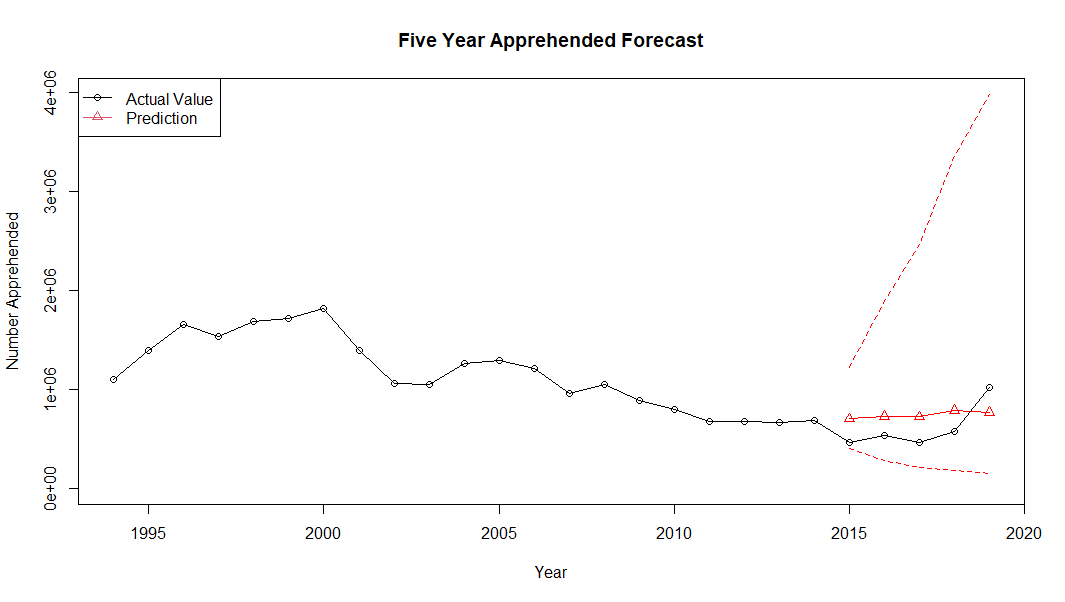
\includegraphics[scale=0.3]{images/NumApp_forecast.png}
\caption{Forecast Plot of logapp ARMA(0,1,12) Model with significant coefficients}
\label{fig:forecast numapp}
\end{figure}

\subsection{Number Removed}
After adding back the difference order, the only model that was worth checking was ARIMA(3,1,3), which has an AIC value of -0.7. \\ 

\begin{verbatim}
Call:
arima(x = logrem, order = c(3, 1, 3))

Coefficients:
         ar1     ar2      ar3      ma1      ma2     ma3
      0.5625  0.0256  -0.7593  -0.3872  -0.2082  0.8570
s.e.  0.1445  0.1927   0.1396   0.1212   0.1517  0.1394

sigma^2 estimated as 0.05002:  log likelihood = 6.35,  aic = 1.3
\end{verbatim}

These are the significant coefficients: \\

\begin{verbatim}
z test of coefficients:

Estimate Std. Error z value  Pr(>|z|)    
ar1  0.562496   0.144501  3.8927 9.914e-05 ***
ar2  0.025558   0.192660  0.1327  0.894464    
ar3 -0.759337   0.139646 -5.4376 5.400e-08 ***
ma1 -0.387202   0.121248 -3.1935  0.001406 ** 
ma2 -0.208241   0.151683 -1.3729  0.169792    
ma3  0.857048   0.139368  6.1495 7.770e-10 ***
---
Signif. codes:  0 ‘***’ 0.001 ‘**’ 0.01 ‘*’ 0.05 ‘.’ 0.1 ‘ ’ 1
\end{verbatim}

Since removing the non-significant coefficients increased the AIC value, no coefficients were removed. \\

$( 1 + 0.9399 B_2  - 0.2035 B_3 ) ( 1 – B )1 X_t = ( 1 + 0.1427 B + B_2)\epsilon_t$

\begin{figure}[h!]
\centering
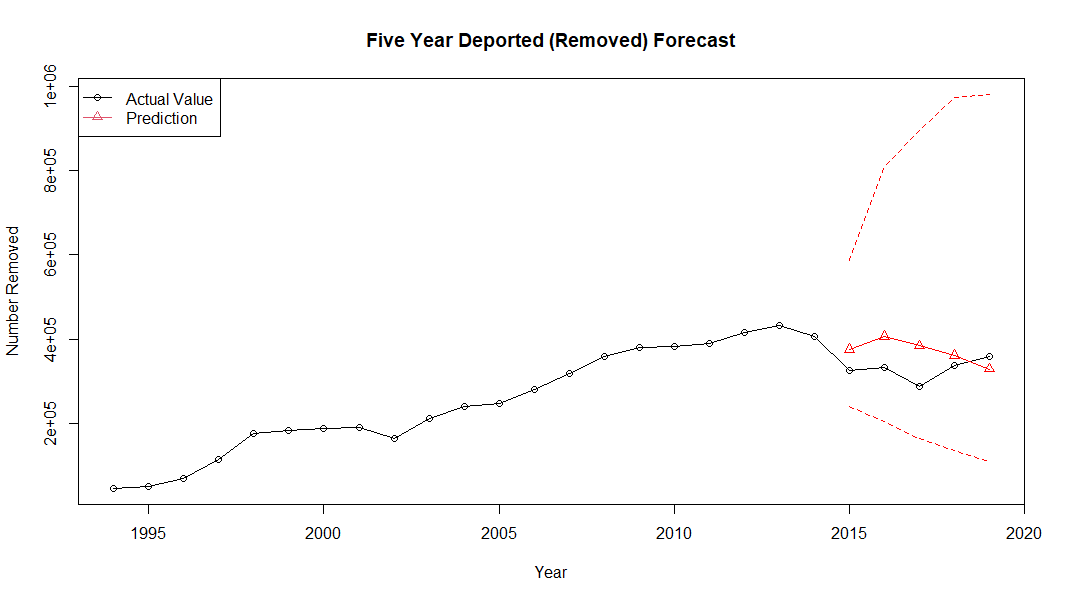
\includegraphics[scale=0.3]{images/Numrem_forecast.png}
\caption{Forecast Plot of logrem ARMA(3,1,3) Model}
\label{fig:forecast numrem}
\end{figure}

\subsection{Number Returned}
After adding back the difference order, the only model to check was ARIMA(1,1,0). \\

\begin{verbatim}
Call:
arima(x = new_logret, order = c(1, 1, 0))

Coefficients:
         ar1
      0.4556
s.e.  0.0948

sigma^2 estimated as 0.09007:  log likelihood = -18.85,  aic = 39.7
> 
\end{verbatim}

This model had an AIC value of 39.7 with the the significant coefficients listed as: \\ 

\begin{verbatim}
z test of coefficients:

Estimate Std. Error z value  Pr(>|z|)    
ar1 0.455631   0.094818  4.8053 1.545e-06 ***
---
Signif. codes:  0 ‘***’ 0.001 ‘**’ 0.01 ‘*’ 0.05 ‘.’ 0.1 ‘ ’ 1

\end{verbatim}

$\hat{Y}_t = µ + Y_(t-1) +  0.4556 ( Y_(t-1) – Y_(t-2))$

\begin{figure}[h!]
\centering
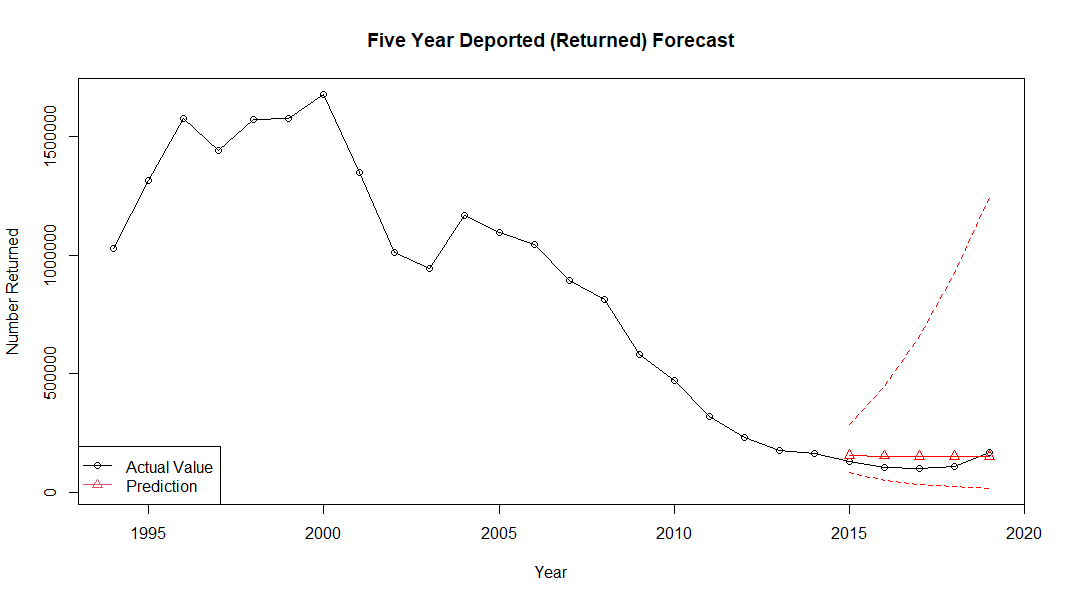
\includegraphics[scale=0.3]{images/numret_forecast.png}
\caption{Forecast Plot of logret ARMA(1, 1, 0) Model}
\label{fig:forecast numret}
\end{figure}


\section{Intervention Events}
Before analyzing interventions, we need to identify the significant outliers. We first perform the locate.outliers function in R on the residuals of our three models. \\

For our selected app model, no outliers were identified in the residual data. However, for the deported models (rem and ret), a few outliers were found: \\

\textbf{Residual Outliers from Selected rem Model}
\begin{verbatim}
  type ind    coefhat     tstat
1   AO  26 -0.6373329 -3.696818
2   AO  58 -0.8493135 -4.765517
3   TC  63 -0.5904907 -3.897957
\end{verbatim}

\textbf{Residual Outliers from Selected ret Model}
\begin{verbatim}
  type ind    coefhat     tstat
1   AO   3 -0.9314625 -5.350058
2   AO  27  0.6879634  3.951468
5   TC  16  0.7165402  3.939461
6   TC  17  0.7910875  4.349314
7   TC  28 -1.4838573 -8.158088
\end{verbatim}

Both datasets have different indexes since the ret dataset has less rows. However, at point 63 for the rem dataset and at point 28 for ret dataset, they both appear to be outliers for the year 1953.

\subsection{Operation Wetback}

Around 1953, the Bracero program was in full swing which allowed Mexican laborers to work in the U.S. for in exchange stricter border security and the return of illegal Mexican immigrants. However, the program did not work since more American growers continued to recruit illegal immigrants for work. A lot of Mexican laborers took the opportunity to move to the U.S. because of the food shortages at home. \\

Eventually many prominent Mexican farm owners were unhappy of the situation since they were losing potential workers to the U.S. So they applied pressure to the Mexican government to address the problem who went to the U.S. government to discuss solutions. One of these solutions was Operation Wetback. \\

Operation Wetback is an immigration enforcement initiative set in June 1954 that used military-style tactics to remove Mexican immigrants from the U.S. So it makes sense that the year before Operation Wetback was initiated, the the records show a spike in the number of removed and returned immigrants. Thus, for our intervention analysis we will look into the year 1953 for the rem and ret dataset.

\subsection{Select the Best Intervention}

The locate.outliers function recognize the outlier type at 1953 for the rem and ret dataset as "TC" or "Temporary Change". However, before we assume the intervention is only temporary, we can check by creating a variety of ARIMAX models with the following intervention conditions:

\begin{itemize}
    \item None
    \item Temporary Intervention
    \item Permanent Intervention
    \item Temporary and Permanent Intervention
\end{itemize}

After the ARIMAX models are created, we can select the best one with the lowest AIC value. Table \ref{tab:aic4} lists each rem intervention along with its AIC value. The best model to proceed forward in plotting its total impact is the temporary and permanent intervention.

\begin{table}[h!]
    \centering
    \caption{Intervention Analysis on the rem Dataset}
    \begin{tabular}{|c|c|c|}
    \hline
    Intervention & AIC & Model Selected? \\
    \hline
    None & 26.95 & No \\ 
    \hline
    Temporary & 28.57 & No \\
    \hline
    Permanent & 26.44 & No \\
    \hline
    Temporary \& Permanent & 22.34 & Yes \\
    \hline
    \end{tabular}
    \label{tab:aic4}
\end{table}

As for the ret dataset, we plot a similar table that lists the interventions and its AIC values (Table \ref{tab:aic5}). However, the best model selected for this case is only the permanent intervention.

\begin{table}[h!]
    \centering
    \caption{Intervention Analysis on the ret Dataset}
    \begin{tabular}{|c|c|c|}
    \hline
    Intervention & AIC & Model Selected? \\
    \hline
    None & 39.38 & No \\ 
    \hline
    Temporary & 20.82 & No \\
    \hline
    Permanent & 18.89 & Yes \\
    \hline
    Temporary \& Permanent & NaN & No \\
    \hline
    \end{tabular}
    \label{tab:aic5}
\end{table}

\subsection{Total Impact}
The total impact shows the effect of an outlier from that point on and out. Even though the 1953 outlier was a temporary change for both the rem and ret datsets (as reflected in the time series plot and the locate.outliers function), the intervention overall reflects a more permanent change. This can be seen in our total impact plots in Figure \ref{fig:int_rem} and \ref{fig:int_ret}. \\

\begin{figure}[h!]
\centering
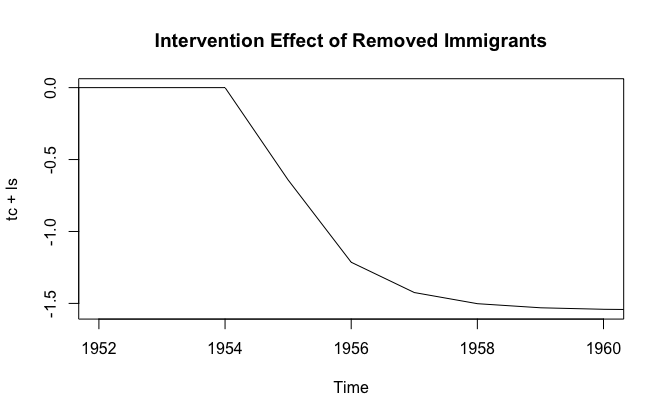
\includegraphics[scale=0.4]{images/int_rem}
\caption{Total Impact Plot of rem}
\label{fig:int_rem}
\end{figure}

\begin{figure}[h!]
\centering
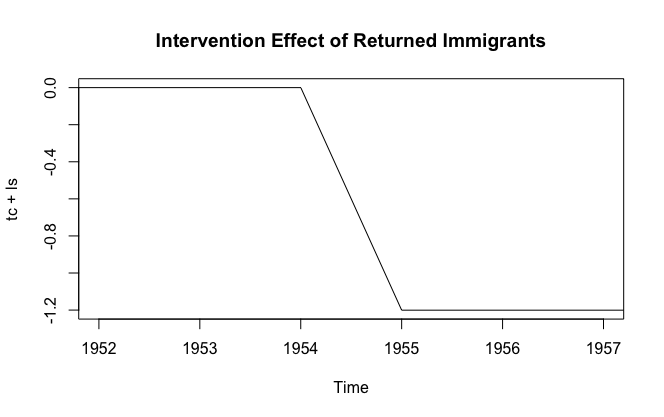
\includegraphics[scale=0.4]{images/int_ret.png}
\caption{Total Impact Plot of ret}
\label{fig:int_ret}
\end{figure}

The intervention analysis overall is valid since it shows how Operation Wetback set a precedence in the following years regarding immigration policy. It may have not been an instant change, but an upward trend took shape around the 1980s when more immigration policies were created.

\section{Multivariate Time Series Analysis}
Since num, rem, and ret have no causal relationship, a multivariate time series analysis is considered over a time series regression. We can begin by creating a vector autoregresssion (VAR) model with the p order at one. A VAR model essentially extends the idea of a univariate AR model to a multivariate time series regression. \\

To determine the best p order before creating a VAR model, we can call for the VARselect function in R. Based on the output, the optimum p order is  one. \\

When calling the VAR function in R with $p=1$, we get the following output:

\begin{verbatim}
VAR Estimation Results:
========================= 
Endogenous variables: num, rem, ret 
Deterministic variables: const 
Sample size: 92 
Log Likelihood: -3387.267 
Roots of the characteristic polynomial:
0.9895 0.9672 0.9672
Call:
VAR(y = x, p = 1)


Estimation results for equation num: 
==================================== 
num = num.l1 + rem.l1 + ret.l1 + const 

         Estimate Std. Error t value Pr(>|t|)    
num.l1     1.2524     0.2021   6.198  1.8e-08 ***
rem.l1    -0.3253     0.2213  -1.470   0.1452    
ret.l1    -0.3183     0.2093  -1.521   0.1318    
const  48449.0075 28250.4532   1.715   0.0899 .  
---
Signif. codes:  0 ‘***’ 0.001 ‘**’ 0.01 ‘*’ 0.05 ‘.’ 0.1 ‘ ’ 1


Residual standard error: 173400 on 88 degrees of freedom
Multiple R-Squared: 0.901,	Adjusted R-squared: 0.8976 
F-statistic: 266.8 on 3 and 88 DF,  p-value: < 2.2e-16 


Estimation results for equation rem: 
==================================== 
rem = num.l1 + rem.l1 + ret.l1 + const 

         Estimate Std. Error t value Pr(>|t|)    
num.l1 -5.107e-02  1.893e-02  -2.697  0.00839 ** 
rem.l1  1.052e+00  2.074e-02  50.697  < 2e-16 ***
ret.l1  6.216e-02  1.961e-02   3.170  0.00210 ** 
const  -1.640e+03  2.647e+03  -0.619  0.53724    
---
Signif. codes:  0 ‘***’ 0.001 ‘**’ 0.01 ‘*’ 0.05 ‘.’ 0.1 ‘ ’ 1


Residual standard error: 16240 on 88 degrees of freedom
Multiple R-Squared: 0.9843,	Adjusted R-squared: 0.9837 
F-statistic:  1836 on 3 and 88 DF,  p-value: < 2.2e-16 


Estimation results for equation ret: 
==================================== 
ret = num.l1 + rem.l1 + ret.l1 + const 

         Estimate Std. Error t value Pr(>|t|)   
num.l1     0.3402     0.1861   1.828  0.07087 . 
rem.l1    -0.5258     0.2038  -2.580  0.01154 * 
ret.l1     0.6047     0.1927   3.138  0.00231 **
const  42057.5345 26011.1872   1.617  0.10948   
---
Signif. codes:  0 ‘***’ 0.001 ‘**’ 0.01 ‘*’ 0.05 ‘.’ 0.1 ‘ ’ 1


Residual standard error: 159600 on 88 degrees of freedom
Multiple R-Squared: 0.902,	Adjusted R-squared: 0.8986 
F-statistic: 269.9 on 3 and 88 DF,  p-value: < 2.2e-16 



Covariance matrix of residuals:
          num       rem       ret
num 3.005e+10 1.018e+09 2.569e+10
rem 1.018e+09 2.639e+08 5.937e+08
ret 2.569e+10 5.937e+08 2.548e+10

Correlation matrix of residuals:
       num    rem    ret
num 1.0000 0.3616 0.9286
rem 0.3616 1.0000 0.2290
ret 0.9286 0.2290 1.0000
\end{verbatim}

Based on the first part of the VAR output regarding estimation results, the num variable only has one significant coefficient. That coefficient is itself. As for the rem dataset, all the variables have significant coefficients along with itself. The ret dataset though only has significant coefficients with the rem variable and itself. \\

For the covariance and correlation matrix section of the VAR(1) output, there appears to be a stronger relationship between the num and ret dataset. This makes sense considering their time series plot is similar in shape and range. As for rem dataset, it has some relationship with num and ret but it is not as strong.

\subsection{Impulse Response Function}
A similar inference from the covariance and correlation matrix can also be observed when plotting the impulse response function (IRF). The x-axis of the plot is standard error, or a unit-less shock value, and the y-axis lists the three datasets response values. The red dotted line is the 95\% confidence interval and red solid horizontal line is where $y=0$. Essentially, the IRF plot shows the response of each dataset when a certain number of shock is applied from one variable. \\

For instance, Figure \ref{fig:irf_num} shows the response of the three variables when a num is applied. As the shock increases, the rem variable is not affected by it compared to the ret variable and itself where the response is decreasing. \\

As for the rem variable in Figure \ref{fig:irf_rem}, there is not a strong response from any of the variables since the plot is close to 0 (solid red line). \\

In Figure \ref{fig:irf_ret}, the ret IRF plot is similar to the num IRF plot. The ret variable decreases the response of itself and the num variable. \\

When analyzing the relationship between num and ret we can infer that if more immigrants are apprehended, then more immigrants are in the "system". This means undocumented immigrants may find it difficult to go through the immigration court process if there’s more people in queue. So most likely, they may decide to return back to their country if that's the case.

\begin{figure}[h!]
\centering
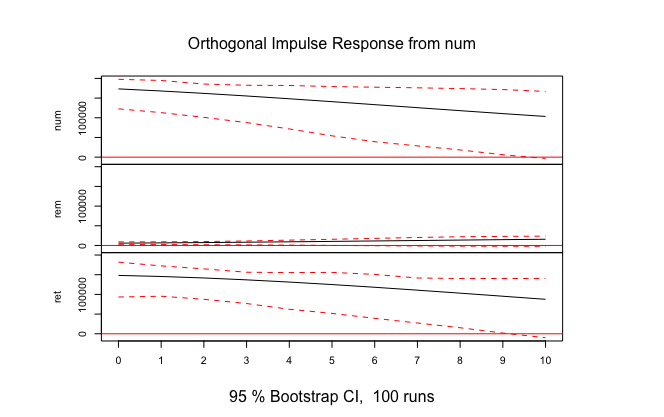
\includegraphics[scale=0.4]{images/irf_num.png}
\caption{IRF of num}
\label{fig:irf_num}
\end{figure}

\begin{figure}[h!]
\centering
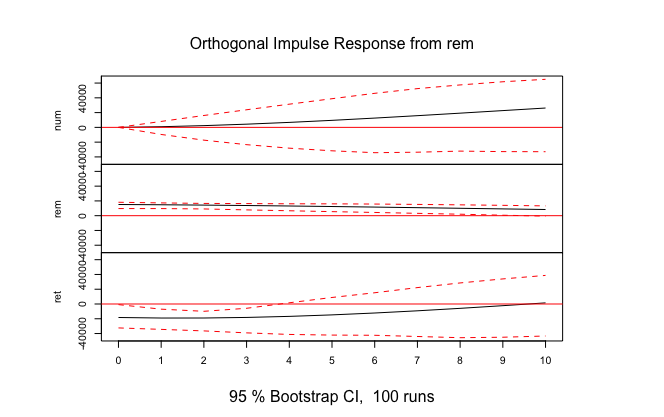
\includegraphics[scale=0.4]{images/irf_rem.png}
\caption{IRF of rem}
\label{fig:irf_rem}
\end{figure}

\begin{figure}[h!]
\centering
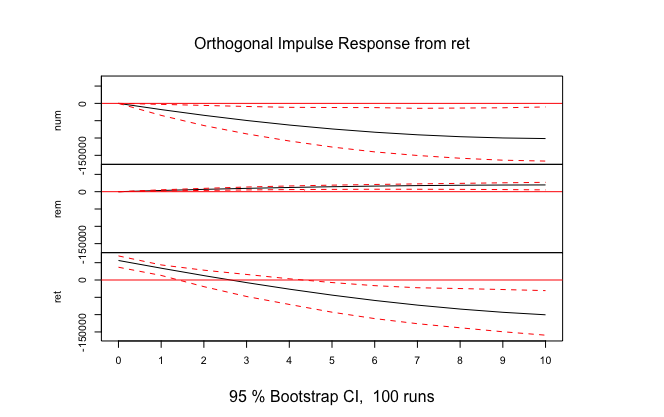
\includegraphics[scale=0.4]{images/irf_ret.png}
\caption{IRF of ret}
\label{fig:irf_ret}
\end{figure}

\subsection{Portmanteau Test}
The Portmanteau test for VAR models is similar to the Box-Ljung test for ARIMA models. The Portmanteau test determines if the VAR model's residuals are white noise. Here's the conditions of the test:

\begin{itemize}
    \item \underline{$H_0$}: Variable residuals are not serially correlated (white noise)
    \item \underline{$H_a$}: Variable residuals are serially correlated (not white noise)
    \item \underline{Condition}: Reject $H_0$ if p-value is less than 0.05. This means if the p-value is greater than 0.05 the residuals are white noise and the variables are not serially correlated.
\end{itemize}

Since the p-value of the VAR(1) model is 0.4004, the residuals are deemed white noise and the variables are not serially correlated.
\end{document}